\documentclass[12pt]{article}

%%%%%%%%%%%%%%%%%%%%%%%%%%%%%%%%%%%%%%%%%%%%%%%%%%%%%%%%%%%%%%%%%%%%%%%%%%%%%%%%
%                           Package preset for homework
%%%%%%%%%%%%%%%%%%%%%%%%%%%%%%%%%%%%%%%%%%%%%%%%%%%%%%%%%%%%%%%%%%%%%%%%%%%%%%%%
% Miscellaneous
\usepackage[margin=1in]{geometry}
\usepackage[utf8]{inputenc}
\usepackage{indentfirst}
\usepackage{blindtext}
\usepackage{graphicx}
\usepackage{xr-hyper}
\usepackage{hyperref}
\usepackage{enumitem}
\usepackage{color}
\usepackage{float}
% Math
\usepackage{latexsym}
\usepackage{amsfonts}
\usepackage{amssymb}
\usepackage{amsmath}
\usepackage{commath}
\usepackage{amsthm}
\usepackage{bbold}
\usepackage{bm}
% Physics
\usepackage{physics}
\usepackage{siunitx}
% Code typesetting
\usepackage{listings}
% Citation
\usepackage[authoryear]{natbib}
\usepackage{appendix}
\usepackage[capitalize]{cleveref}
% Title & name
\title{Homework}
\author{Tien Vo}
\date{\today}


%%%%%%%%%%%%%%%%%%%%%%%%%%%%%%%%%%%%%%%%%%%%%%%%%%%%%%%%%%%%%%%%%%%%%%%%%%%%%%%%
%                   User-defined commands and environments
%%%%%%%%%%%%%%%%%%%%%%%%%%%%%%%%%%%%%%%%%%%%%%%%%%%%%%%%%%%%%%%%%%%%%%%%%%%%%%%%
%%% Misc
\sisetup{load-configurations=abbreviations}
\newcommand{\due}[1]{\date{Due: #1}}
\newcommand{\hint}{\textit{Hint}}
\let\oldt\t
\renewcommand{\t}[1]{\text{#1}}

%%% Bold sets & abbrv
\newcommand{\N}{\mathbb{N}}
\newcommand{\Z}{\mathbb{Z}}
\newcommand{\R}{\mathbb{R}}
\newcommand{\Q}{\mathbb{Q}}
\let\oldP\P
\renewcommand{\P}{\mathbb{P}}
\newcommand{\LL}{\mathcal{L}}
\newcommand{\FF}{\mathcal{F}}
\newcommand{\HH}{\mathcal{H}}
\newcommand{\NN}{\mathcal{N}}
\newcommand{\ZZ}{\mathcal{Z}}
\newcommand{\RN}[1]{\textup{\uppercase\expandafter{\romannumeral#1}}}
\newcommand{\ua}{\uparrow}
\newcommand{\da}{\downarrow}

%%% Unit vectors
\newcommand{\xhat}{\vb{\hat{x}}}
\newcommand{\yhat}{\vb{\hat{y}}}
\newcommand{\zhat}{\vb{\hat{z}}}
\newcommand{\nhat}{\vb{\hat{n}}}
\newcommand{\rhat}{\vb{\hat{r}}}
\newcommand{\phihat}{\bm{\hat{\phi}}}
\newcommand{\thetahat}{\bm{\hat{\theta}}}

%%% Other math stuff
\providecommand{\units}[1]{\,\ensuremath{\mathrm{#1}}\xspace}
% Set new style for problem
\newtheoremstyle{problemstyle}  % <name>
        {10pt}                   % <space above>
        {10pt}                   % <space below>
        {\normalfont}           % <body font>
        {}                      % <indent amount}
        {\bfseries\itshape}     % <theorem head font>
        {\normalfont\bfseries:} % <punctuation after theorem head>
        {.5em}                  % <space after theorem head>
        {}                      % <theorem head spec (can be left empty, 
                                % meaning `normal')>

% Set problem environment
\theoremstyle{problemstyle}
\newtheorem{problemenv}{Problem}[section]
\newenvironment{problem}[1]{%
  \renewcommand\theproblemenv{#1}%
  \problemenv
}{\endproblemenv}
% Set lemma environment
\newenvironment{lemma}[2][Lemma]{\begin{trivlist}
\item[\hskip \labelsep {\bfseries #1}\hskip \labelsep {\bfseries #2.}]}{\end{trivlist}}
% Set solution environment
\newenvironment{solution}{
    \begin{proof}[Solution]$ $\par\nobreak\ignorespaces
}{\end{proof}}
\numberwithin{equation}{problemenv}

%%% Page format
\setlength{\parindent}{0.5cm}
\setlength{\oddsidemargin}{0in}
\setlength{\textwidth}{6.5in}
\setlength{\textheight}{8.8in}
\setlength{\topmargin}{0in}
\setlength{\headheight}{18pt}

%%% Code environments
\definecolor{dkgreen}{rgb}{0,0.6,0}
\definecolor{gray}{rgb}{0.5,0.5,0.5}
\definecolor{mauve}{rgb}{0.58,0,0.82}
\lstset{frame=tb,
  language=Python,
  aboveskip=3mm,
  belowskip=3mm,
  showstringspaces=false,
  columns=flexible,
  basicstyle={\small\ttfamily},
  numbers=none,
  numberstyle=\tiny\color{gray},
  keywordstyle=\color{blue},
  commentstyle=\color{dkgreen},
  stringstyle=\color{mauve},
  breaklines=true,
  breakatwhitespace=true,
  tabsize=4
}
\lstset{
  language=Mathematica,
  numbers=left,
  numberstyle=\tiny\color{gray},
  numbersep=5pt,
  breaklines=true,
  captionpos={t},
  frame={lines},
  rulecolor=\color{black},
  framerule=0.5pt,
  columns=flexible,
  tabsize=2
}

\usepackage{enumitem}

\title{Homework 6: Phys 7230 (Spring 2022)}
\due{April 25, 2022}

\begin{document}
\maketitle
%%%%%%%%%%%%%%%%%%%%%%%%%%%%%%%%%%%%%%%%%%%%%%%%%%%%%%%%%%%%%%%%%%%%%%%%%%%%%%%
\begin{problem}{1}[Classical 1d Ising model via transfer matrix]
Consider a 1d Ising model with Hamiltonian, $\HH_\t{1d-Ising}=-\sum_{i=1}^N
J\sigma_i\sigma_{i+1}$, with nearest neighbords exchange interactions, in zero
external field, and with periodic boundary conditions (i.e., closed spin-1/2
chain on a ring), with $N$ spins and $\sigma_{N+1}=\sigma_1$.

Use transfer matrix methods discussed in the lectures to compute and plot the
total energy $E(T)$ and the corresponding heat capacity $C(T)$, verifying that
they are smooth functions (no singularities) as a function of temperature and
thus demonstrating that classical 1d Ising model exhibits no phase transition
and only has a paramagnetic field.

\textit{Note}: To really show that it is a paramagnet we would need to compute
its magnetization $m(h)$ as a function of field and show that it is always zero
in $h\to0$ limit and exhibits Curie susceptibility of effectively independent
spins. This is worked out in the lecture notes so I will spare you the extra
work, but encourage you to explore it furter if you are interested.
\begin{solution}
Given the Hamiltonian, the canonical partition function is
\begin{equation}
    Z=\sum_\qty{\sigma_i}\exp\qty(\sum_{i=1}^NJ\sigma_i\sigma_{i+1}) 
    =\sum_\qty{\sigma_i}T_{\sigma_1\sigma_2}T_{\sigma_2\sigma_3}\hdots
    T_{\sigma_N\sigma_1}
    =\tr[\hat{T}^N],
\end{equation}
where $\beta J\mapsto J$ and
\begin{equation}
    \hat{T}_{\sigma\sigma'}=e^{J\sigma\sigma'}=\mqty(e^J&e^{-J}\\e^{-J}&e^J).
\end{equation}
The eigenvalues of $\hat{T}$ are roots of the characteristic polynomial
\begin{equation}
    \det\qty(\hat{T}-\lambda\mathbb{1}) 
    =\det\mqty(e^{J}-\lambda&e^{-J}\\e^{-J}&e^J-\lambda)
    =\lambda^2-2\lambda e^J+e^{2J}-e^{-2J}=0,
\end{equation}
which are $\lambda_\pm=e^J\pm e^{-J}$. Thus, it follows that
\begin{equation}
    Z=\lambda_+^N+\lambda_-^N=\qty(2\cosh J)^N+\qty(2\sinh
    J)^N=\qty(2\cosh(\beta J))^N+(2\sinh(\beta J))^N
    \approx (2\cosh(\beta J))^N,
\end{equation}
where we have unpacked $J$ back into units of energy in the last equality and
assumed the thermodynamic limit $N\gg 1$. Now, by definition, the energy is
\begin{equation}
    E(T)=-\frac{\partial\ln Z}{\partial\beta}
    =-NJ\tanh(\beta J).
\end{equation}
Also, the heat capacity is
\begin{equation}
    C_V(T)=\frac{\partial E}{\partial T}
    =-k_B\beta^2\frac{\partial E}{\partial\beta}=Nk_B(\beta J)^2\sech^2(\beta
    J).
\end{equation}
Letting the crossover temperature be $T_\ast=J/k_B$, these results can be
rewritten as
\begin{equation}
    E(T)=-Nk_BT_\ast\tanh\qty(\frac{T_\ast}{T}),\qquad\t{and}\qquad
    C_V(T)=Nk_B\qty(\frac{T_\ast}{T})^2\sech^2\qty(\frac{T_\ast}{T}).
\end{equation}
A plot of them is included below. As expected, $E\to0$ at high temperature and
saturates at $-Nk_BT_\ast$ at low temperature, and $C_v$ exhibits the Schottky
peak form, which crosses over at $T=T_\ast$.
\begin{center}
    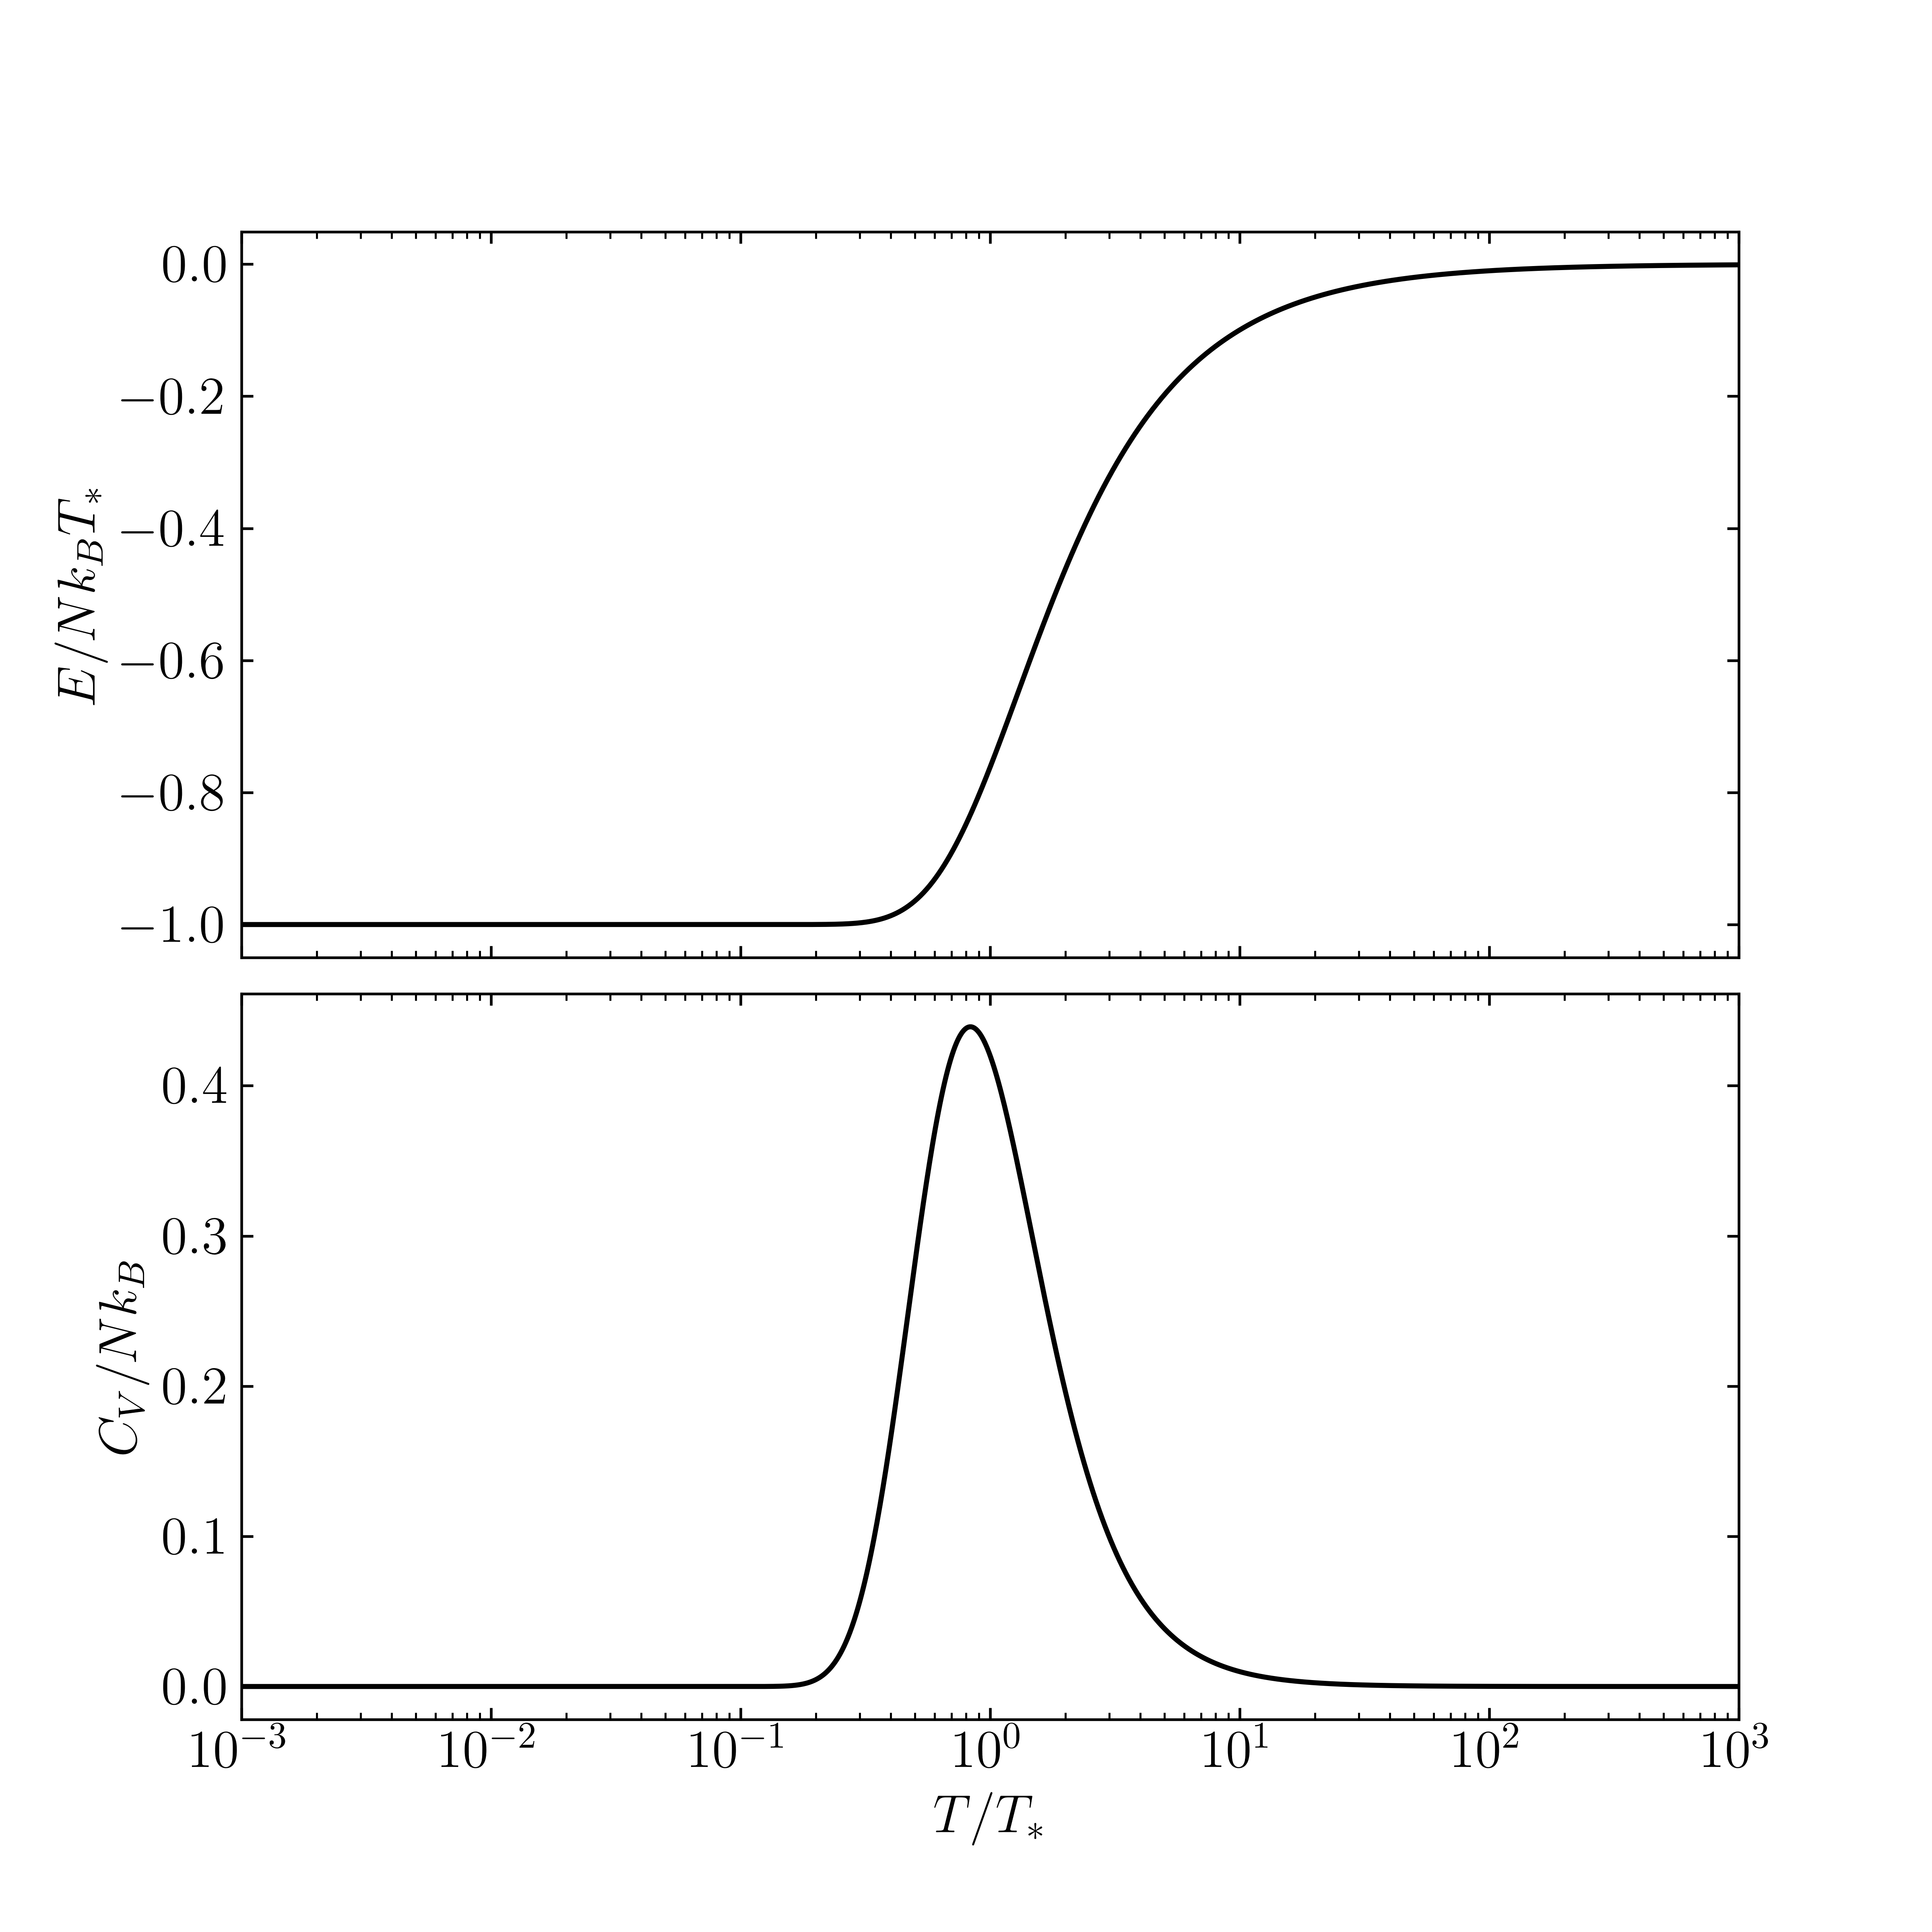
\includegraphics[width=0.8\textwidth]{p1.png} 
\end{center}
\end{solution}
\end{problem}
\newpage
%%%%%%%%%%%%%%%%%%%%%%%%%%%%%%%%%%%%%%%%%%%%%%%%%%%%%%%%%%%%%%%%%%%%%%%%%%%%%%%    
%%%%%%%%%%%%%%%%%%%%%%%%%%%%%%%%%%%%%%%%%%%%%%%%%%%%%%%%%%%%%%%%%%%%%%%%%%%%%%%
\begin{problem}{2}[Ising model in a field via Weiss mean-field theory]~\\

(a) Estimate very roughly the strength of Coulomb interaction in solids, thereby
verifying that $E_\t{Coulomb}\gg E_\t{dipole}$, comparing it also to room
temperature. (\textit{Hint}: no complicated calculations are really needed, just
reference to a familiar result in e.g., quantum mechanics, where you know the
result well in \si{eV}).
\begin{solution}
The Coulomb potential energy is
\begin{equation}
    E_\t{Coulomb}=\frac1{4\pi\epsilon_0}\frac{e^2}{r_0}\approx 27\,\si{eV},
\end{equation}
where $e$ is the charge of an electron and $r_0$ is the Bohr radius. Thus,
compared to $E_\t{dipole}\approx10^{-4}\,\si{eV}$, the Coulomb interaction
dominates in a solid. This is also much larger than thermal motion at room
temperature $k_BT\sim0.03\,\si{eV}$.
\end{solution}

(b) Using Weiss mean-field approximation, rederive the implicit self-consistent
MFT equation for the magnetization in $m(T,B)$.
\begin{solution}
First, the classical Heisenberg Hamiltonian with external field is
\begin{equation}\label{p2b:H}
    \HH=-\frac12\sum_{ij}J_{ij}\vb{S}_i\vdot\vb{S}_j-\mu\vb{S}\vdot\vb{B}.
\end{equation}
Now, we write $\vb{S}_i=\expval{\vb{S}_i}+\delta\vb{S}_i$, where
$\delta\vb{S}_i=\vb{S}_i-\expval{\vb{S}_i}$. Plugging this into \eqref{p2b:H},
ignoring the $\order{\delta\vb{S}^2}$ terms, we get
\begin{align}
    \HH
    &=-\frac12\sum_{ij}J_{ij}\expval{\vb{S}_i}\vdot\expval{\vb{S}_j}
    -\frac12\sum_{ij}J_{ij}(\expval{\vb{S}_i}\vdot\delta\vb{S}_j+\expval{\vb{S}_j}\vdot\delta\vb{S}_i)-\mu\vb{B}\vdot\sum_i\vb{S}_i\notag\\
    &=-\frac12\sum_{ij}J_{ij}\expval{\vb{S}_i}\vdot\expval{\vb{S}_j}
    -\sum_{ij}J_{ij}\expval{\vb{S}_j}\vdot\qty(\vb{S}_i-\expval{\vb{S}_i})
    -\mu\vb{B}\vdot\sum_i\vb{S}_i\notag\\
    &=\frac12\sum_{ij}J_{ij}\expval{\vb{S}_i}\vdot\expval{\vb{S}_j}
    -\sum_{ij}J_{ij}\expval{\vb{S}_j}\vdot\vb{S}_i-\mu\vb{B}\vdot\sum_i\vb{S}_i,
\end{align}
where we have done a label exchange $i\mapsto j$ and $j\mapsto i$ in the second
term in the first equality. Writing the effective Weiss field as
$\vb{B}_\t{eff}=\vb{B}+\frac1\mu\sum_jJ_{ij}\expval{\vb{S}_j}$, we get the same
Hamiltonian (31) in the lecture notes
\begin{align}
    \HH_\t{mft}
    &=\frac12\sum_{ij}J_{ij}\expval{\vb{S}_i}\vdot\expval{\vb{S}_j}-\mu\vb{B}_\t{eff}\vdot\sum_i\vb{S}_i\notag\\
    &=\sum_{i=1}^N\qty[\frac12
    \sum_{j=1}^N\qty(J_{ij}\expval{\vb{S}_i}\vdot\expval{\vb{S}_j})
    -\mu\vb{B}_\t{eff}\vdot\vb{S}_i].
\end{align}
Now, assuming the magnetization doesn't depend on the lattice site
$\vb{m}=n\mu\expval{\vb{S}_i}$, the energy eigenvalues are
\begin{equation}
    E_\t{mft}
    =\sum_{i=1}^N\qty(\frac{\lambda m^2}{2n}-\mu B_\t{eff}s_i),
\end{equation}
where $B_\t{eff}=B+\lambda m$ with $\lambda=J_0/n\mu^2$, $J_0=\sum_{j=1}^N
J_{ij}$, and $s_i\in\qty{-S,-S+1,\hdots,S-1,S}$. The canonical partition function is
\begin{align}
    Z
    &=\prod_{i=1}^N\qty[\sum_{s_i=-S}^S\exp\qty(\frac{-\beta\lambda
    m^2}{2n}+\beta\mu B_\t{eff}s_i)]\notag\\
    &=\qty[\exp\qty(-\frac{\beta \lambda m^2}{2n})\frac{\sinh[(2S+1)\mu
    B_\t{eff}/2k_BT]}{\sinh(\mu B_\t{eff}/2k_BT)}]^N.
\end{align}
The free energy is thus as follows
\begin{equation}\label{p2a:F}
    F=-k_BT\ln Z
    =\frac{N\lambda m^2}{2n}-Nk_BT\ln\qty[\frac{\sinh[(2S+1)\mu
    B_\t{eff}/2k_BT]}{\sinh(\mu B_\t{eff}/2k_BT)}].
\end{equation}
Then, by definition, the magnetization is
\begin{align}
    m
    &=-\frac1V\frac{\partial F}{\partial B}\notag\\
    &=-\lambda m\frac{\partial m}{\partial B}
    -\frac{n\mu}{2}\qty(1+\lambda\frac{\partial m}{\partial B})
    \qty[\coth\qty(\frac{\mu B_\t{eff}}{2k_BT})-(1+2S)\coth\qty[\frac{(1+2S)\mu
B_\t{eff}}{2k_BT}]]\notag\\
    &=-\lambda m\frac{\partial m}{\partial B}
    +n\mu S\qty(1+\lambda\frac{\partial m}{\partial B})
    \Bigg[\qty(1+\frac{1}{2S})\coth\qty[\qty(1+\frac1{2S})\frac{S\mu
    B_\t{eff}}{k_BT}]\notag\\
    &\qquad\qquad-\frac1{2S}\coth\qty(\frac1{2S}\frac{S\mu
B_\t{eff}}{k_BT})\Bigg]\notag\\
    &=-\lambda m\frac{\partial m}{\partial B}
    +n\mu S\qty(1+\lambda\frac{\partial m}{\partial B})
    B_S\qty(\frac{S\mu B_\t{eff}}{k_BT}),
\end{align}
where $B_S$ is the Brillouin function. Simplifying further, we can write a
transcendental equation in $m(T,B)$ as
\begin{equation}\label{p2b:m}
    m=n\mu SB_S\qty(\frac{S\mu B_\t{eff}}{k_BT})
    =n\mu SB_S\qty[\frac{S\mu(B+\lambda m)}{k_BT}].
\end{equation}
\end{solution}

(c) Plot both sides of the MFT equation as a function of $m$ for a range of
$T$'s (i) for $B=0$, thereby solving graphically for $m(T,0)$ demonstrating that
there is a PM-FM phase transition from $m(T>T_c,0)=0$ PM to $m(T<T_c,0)\neq 0$
FM. (ii) Show graphically that for $B\neq 0 $ there is a $m(T,B)\neq 0$ solution
for any finite $T$, and that while for $T>T_c$ this solution is smooth, for
$T<T_c$ it jumps at $B=0$ between $m>0$ to $m<0$, as $B$ changes sign. Thus, for
$T<T_c$ there is a (what's called) a first-order discontinuous phase transition
as a function of $B$ at $B=0$, at which the system jumps between two minima
separated by a barrier. This is in contrast to the continuous second-order
transition as a function of $T$ at $T_c$ for $B=0$, where $m>0$ develops
continuously from $m=0$.
\begin{solution}
(i) For $B=0$, \eqref{p2b:m} becomes
\begin{equation}\label{p2ci:m}
    \frac{m}{n\mu}=SB_S\qty(\frac{3}{S+1}\frac{T_c}{T}\frac{m}{n\mu})
    =SB_S(x), 
\end{equation}
where $T_c=S(S+1)J_0/3k_B$. Below, we plot the LHS (solid red line) and RHS 
(black lines) for three values of $T/T_c$.
\begin{center}
    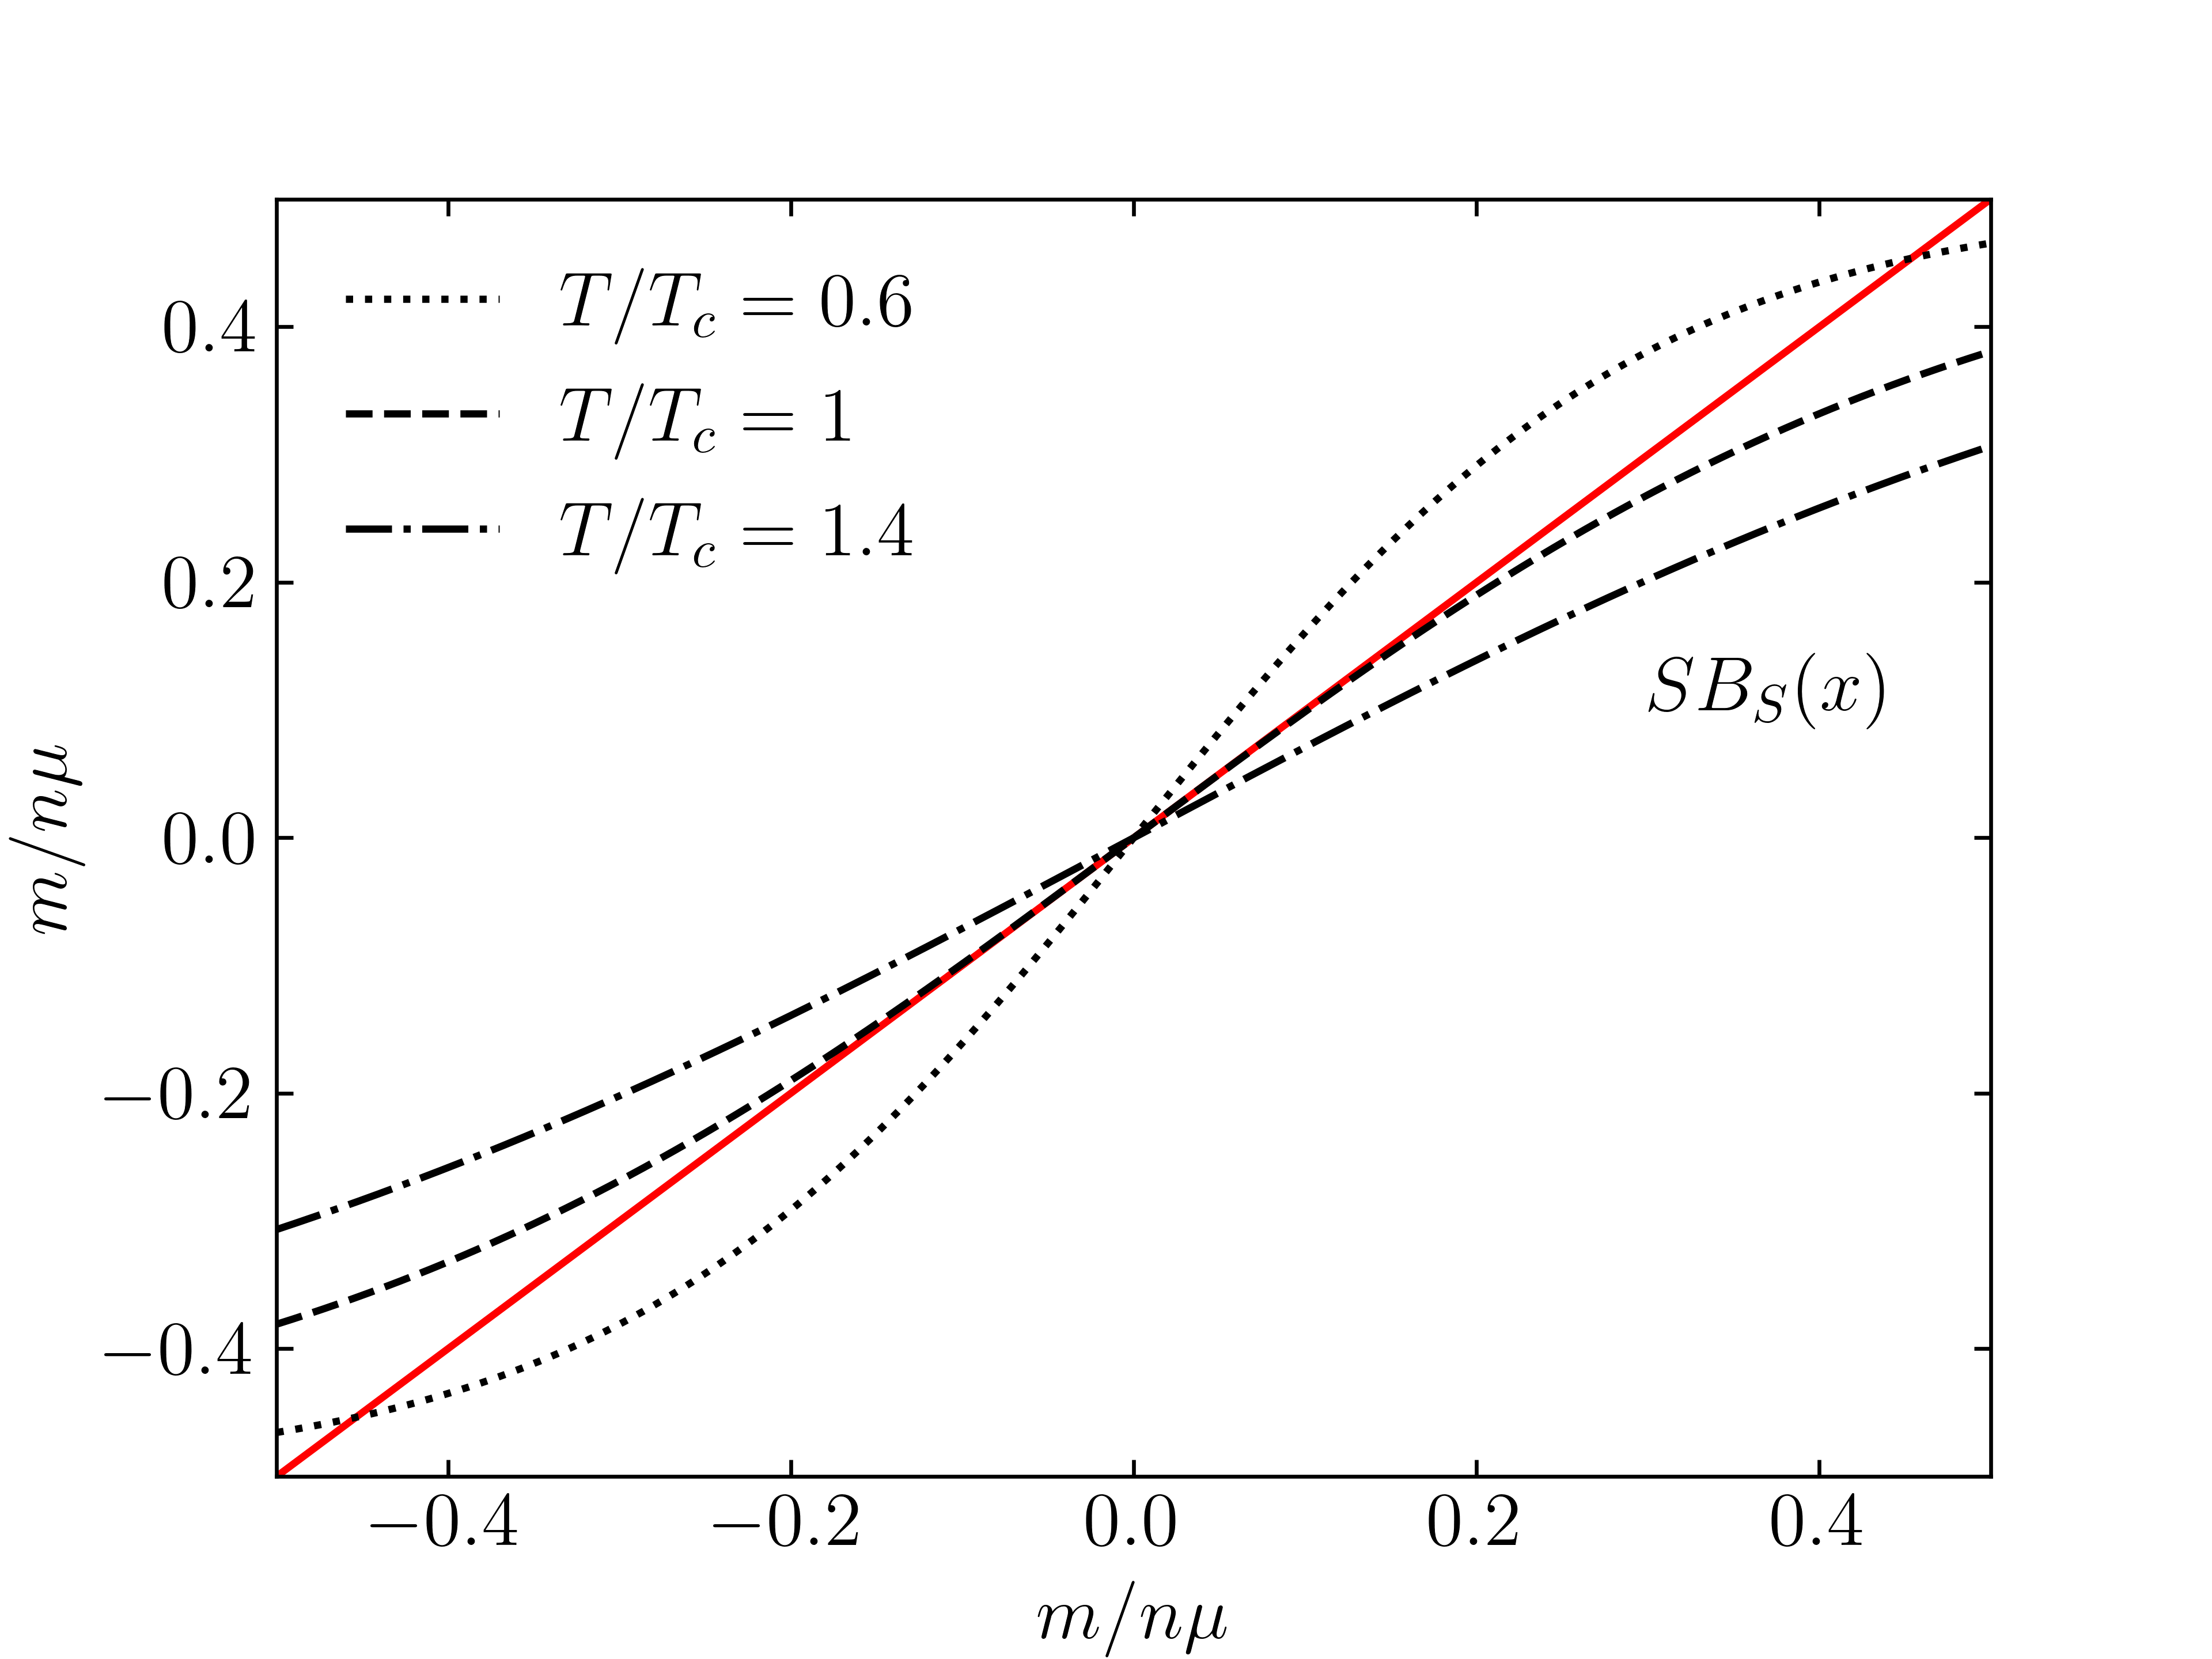
\includegraphics[width=0.8\textwidth]{p2ci.png} 
\end{center}
Thus, \eqref{p2ci:m} has only one root at $m=0$ when $T\geq T_c$ and two extra
non-trivial roots when $T<T_c$. This demonstrates the transition from PM to FM
phase at $T=T_c$.

(ii) Now, for arbitrary $B$, \eqref{p2b:m} is
\begin{equation}
    \frac{m}{n\mu}=SB_S\qty(S\frac{\mu
    B}{k_BT_c}\frac{T_c}{T}+\frac{3}{S+1}\frac{T_c}{T}\frac{m}{n\mu}). 
\end{equation}
With a root-finding algorithm, we can then solve for $m(T,B)/n\mu$ and plot it
below.
\begin{center}
    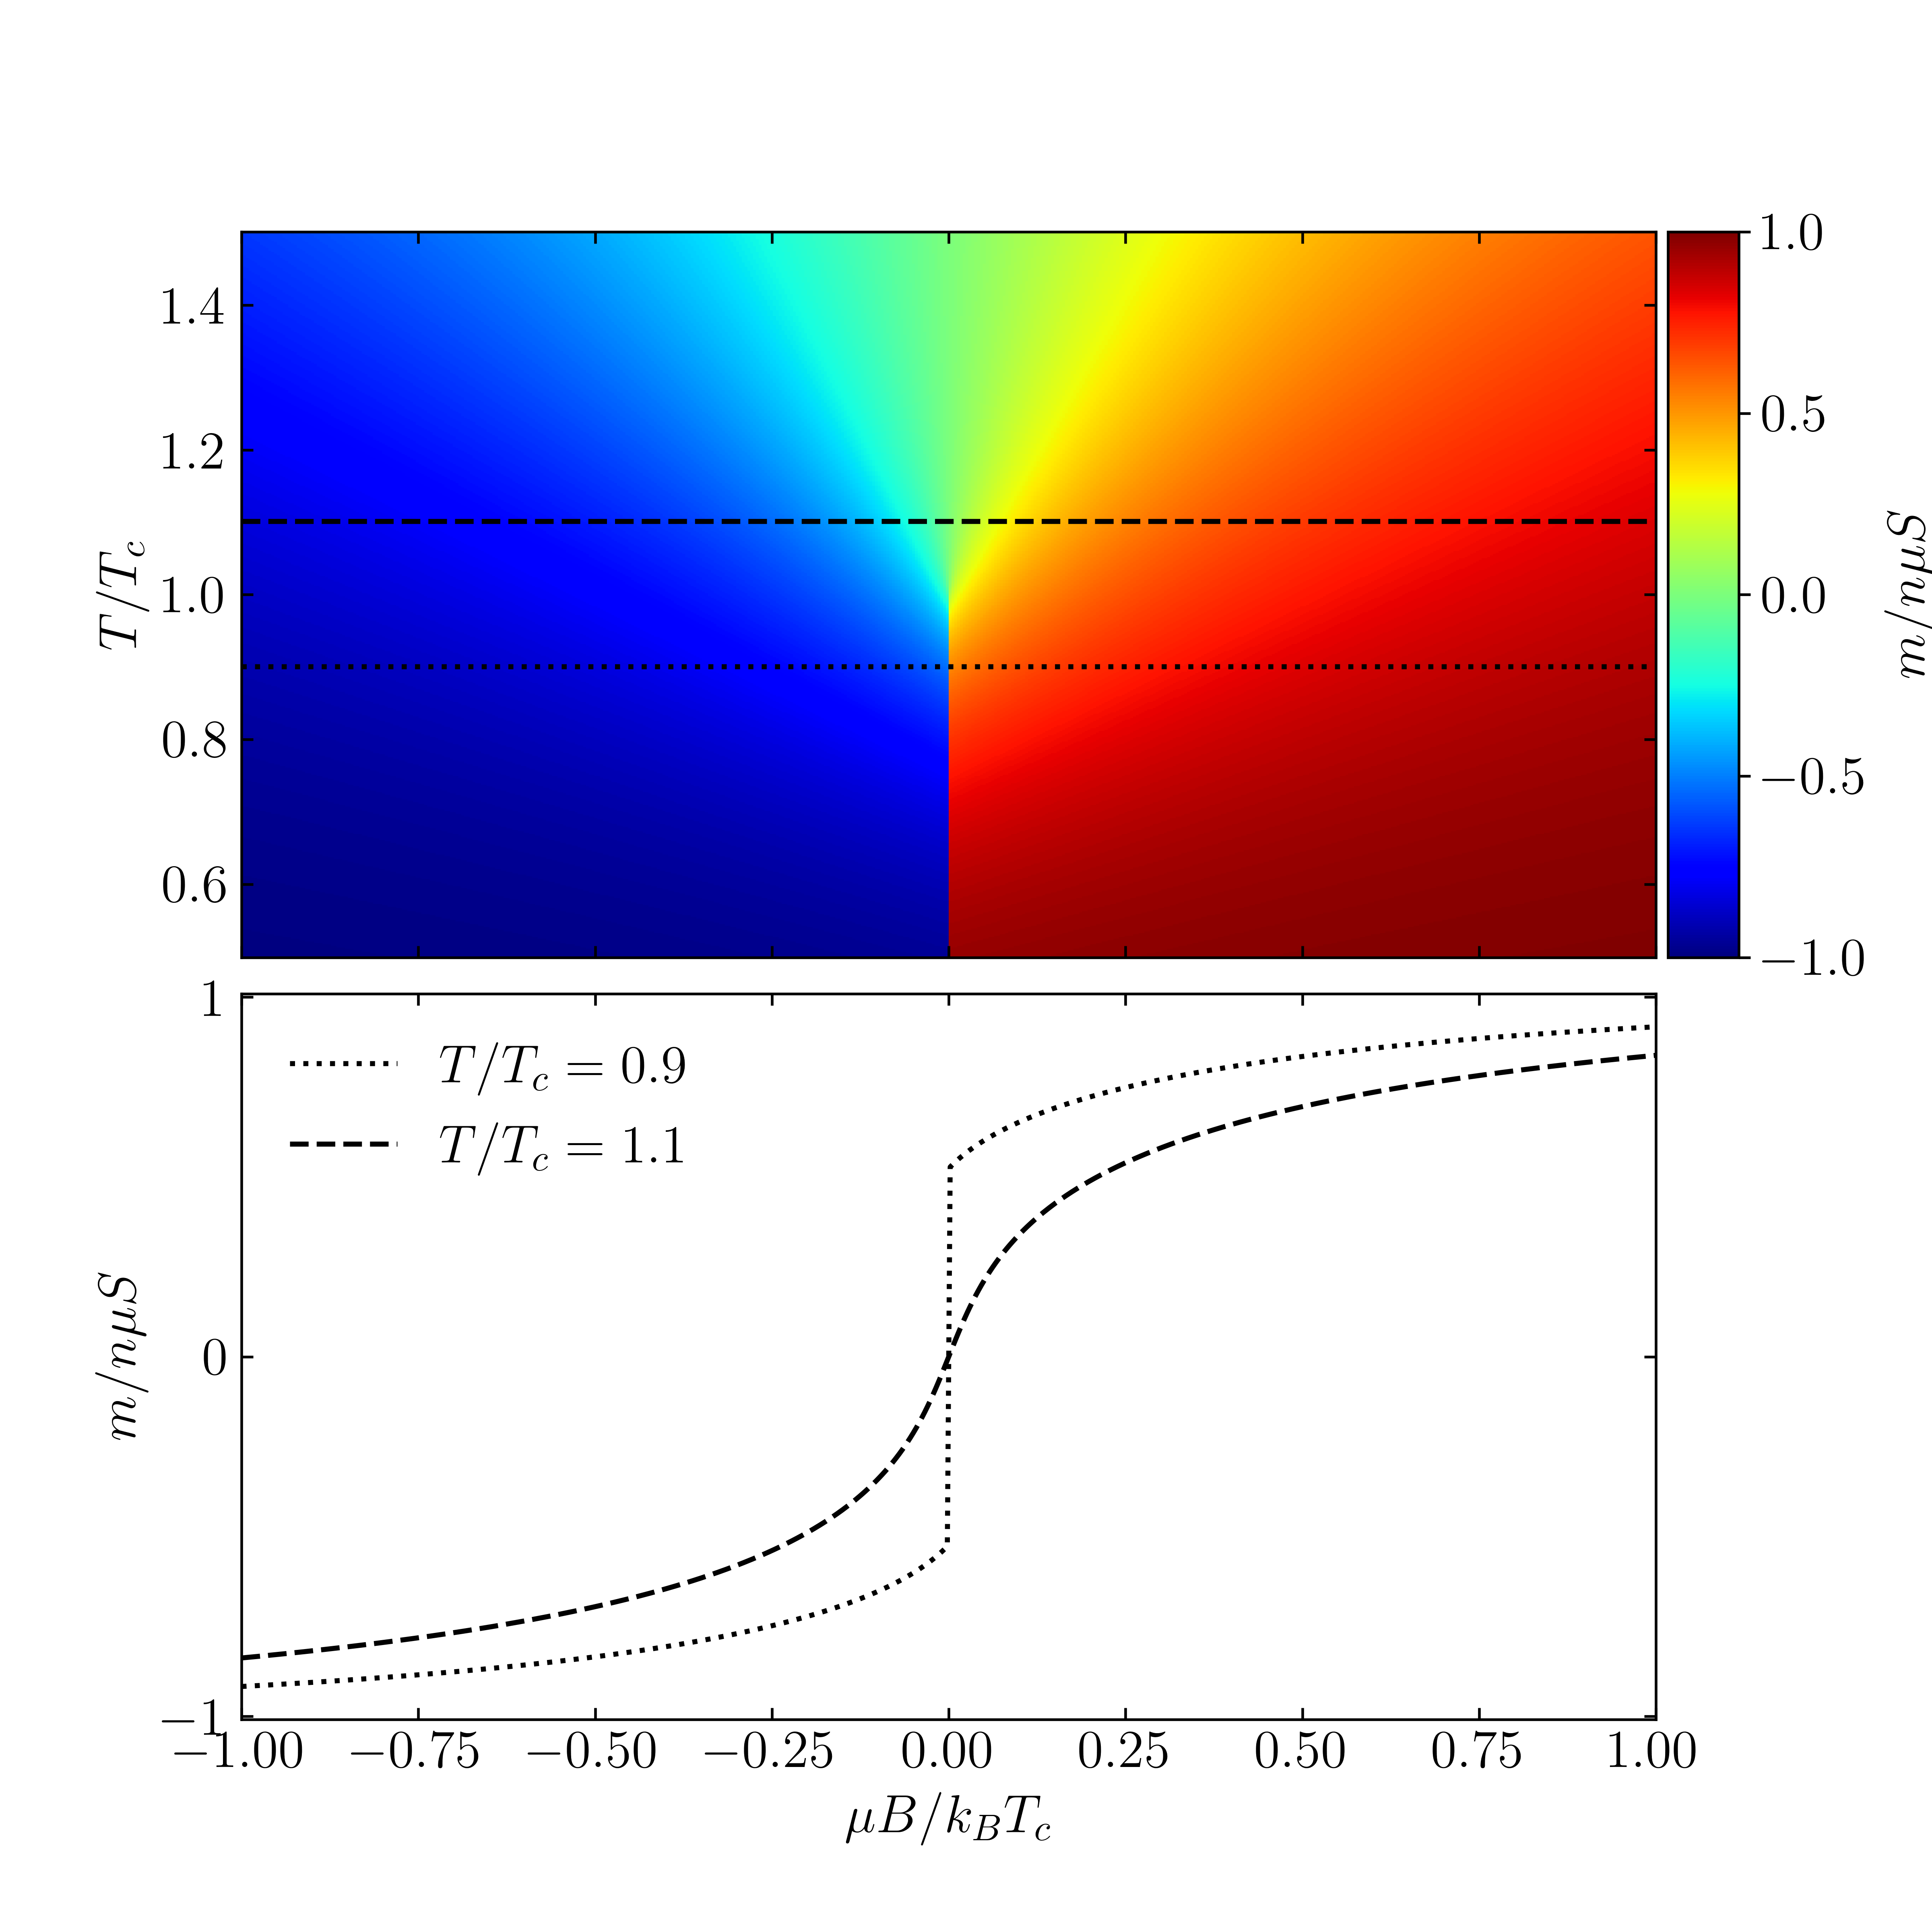
\includegraphics[width=0.8\textwidth]{p2cii.png} 
\end{center}
For $T<T_c$, note that $m$ is discontinuous from $B<0$ ($m=-(1/2)n\mu$) to $B>0$
($m=(1/2)n\mu$), but the solution is smooth for $T\geq T_c$.
\end{solution}

(d) As discussed in the lectures, appreciating that MFT equation for $m$ is
actually a saddle-point equation for free-energy density $f(m,B,T)$ with respect
to $m$, i.e., $\partial f/\partial m=0$, calculate $f(m,B,T)$, plot it for a
range of $T$ and $B$ (including $B=0$), demonstrating how its minima move with
these parameters and thereby showing the PM-FM phase transition and its absence
for $B=0$ and $B\neq 0$, respectively.
\begin{solution}
From \eqref{p2a:F}, we can write
\begin{equation}
    \frac{f}{nk_BT_c}=\frac{F}{Nk_BT_c}
    =\frac{3}{2S(S+1)}\qty(\frac{m}{n\mu})^2-\ln\qty{\frac{\sinh\qty[\qty(1+\frac1{2S})\frac{S\mu
    B_\t{eff}}{k_BT}]}{\sinh\qty(\frac1{2S}\frac{S\mu B_\t{eff}}{k_BT})}},
\end{equation}
where $S\mu B_\t{eff}/k_BT=S(\mu B/k_BT_c)(T_c/T)+3(T_c/T)(m/n\mu)/(S+1)$.
Below, we plot $f(m,B,T)$ for given values of $B$ and $T$.
\begin{center}
    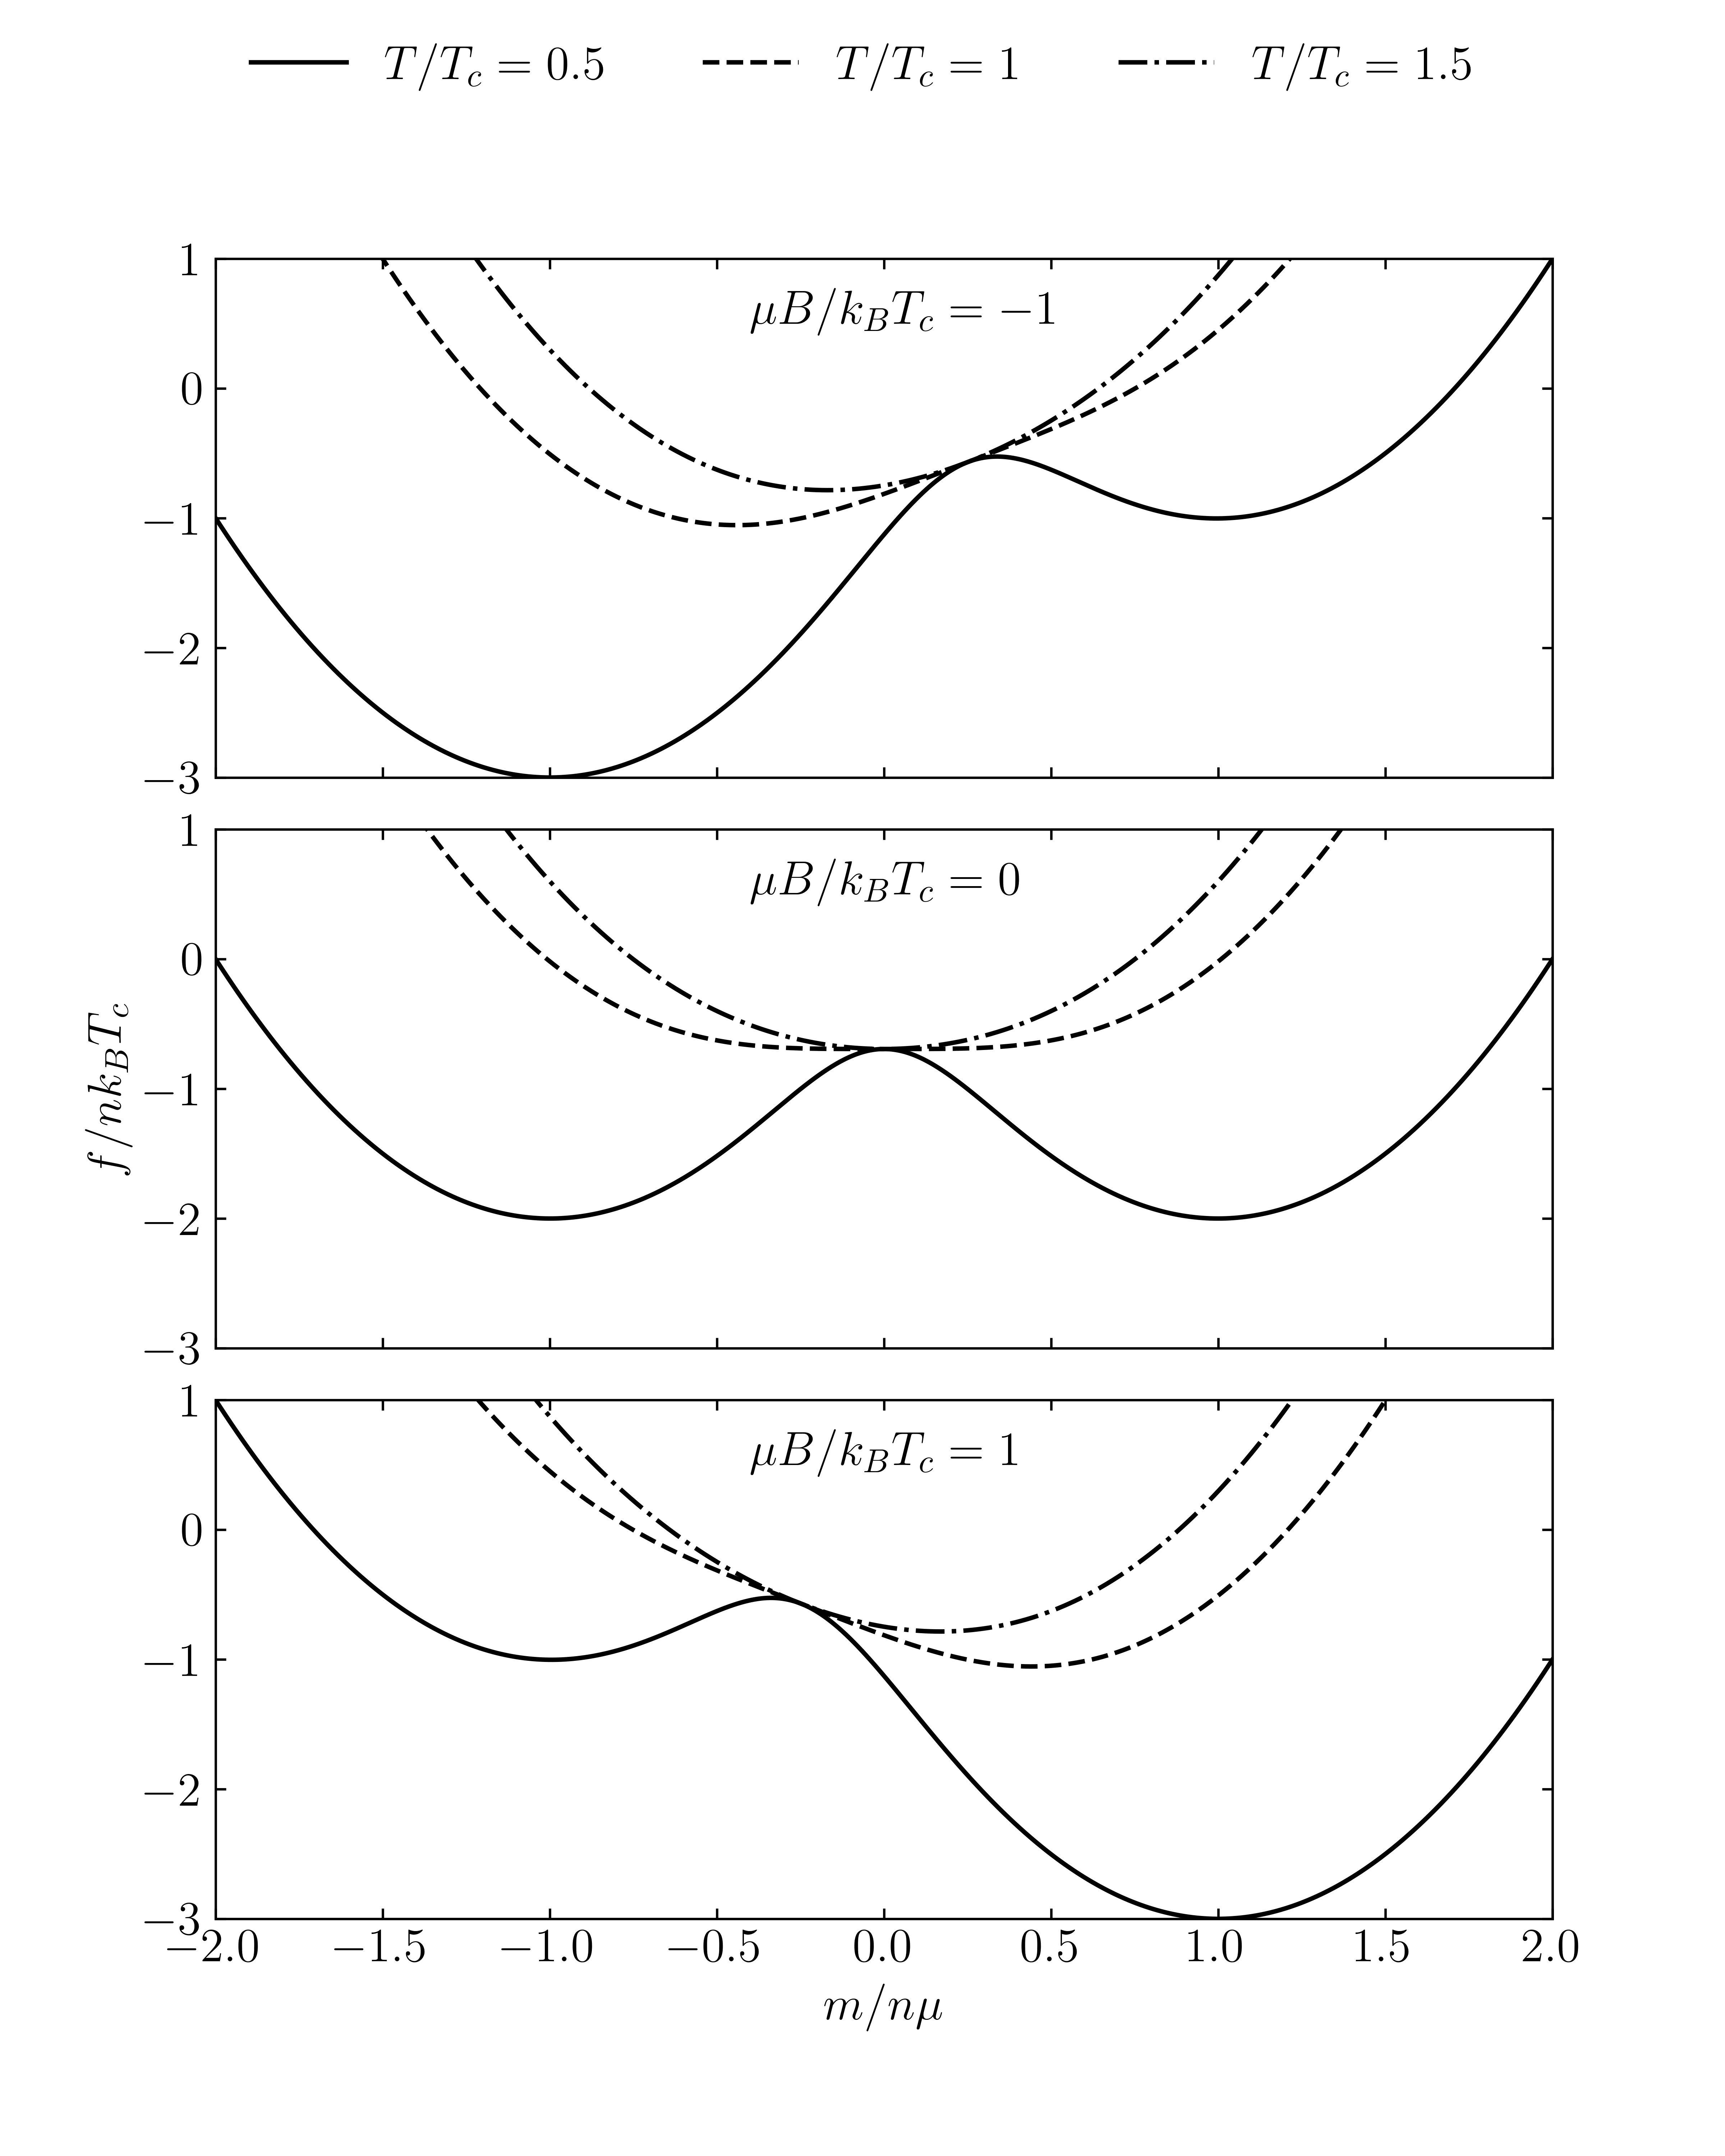
\includegraphics[width=0.8\textwidth]{p2d.png} 
\end{center}
For $B<0$,the minimum of $f$ is always negative for all temperatures $T/T_c$,
moving towards $m=0$ for larger $T$. On the other hand, for $B>0$, the minimum 
of $f$ is always positive. At $B=0$, $f$ only has one minimum for
$T/T_c\geq 1$ at $m=0$, but it has three extrema for $T/T_c<1$, and the one at
$m=0$ is a local maximum.
\end{solution}

(e) By Taylor-expanding $f(m,B,T)$ for small $m$ (in fact it may be more
convenient to expand the saddle-point MFT equation first and then integrate term
by term to obtain the expanded $f(m,B,T)$), show that it exhibits the generic
Landau ``$\phi$'' form (i.e., $m^4$ here, with $\phi=m$) and extract from it the
PM-FM transition temperature $T_c$ in terms of the exchange constant $J_0$.

(f) By minimizing this Landau $\phi^4$ form of $f(m,B,T)$, derive (i) the
spontaneous magnetization $m_0(T<T_c,B=0)$, (ii) $m_0(T_c,B\to0)$, (iii)
$\chi(T)$, thereby extracting the MF critical exponents $\beta,\delta,\gamma$
defined in the lecture notes.

(g) Sketch qualitative behavior of the resulting $m(T,B=0)$ and $m(T,B\neq0)$ as
a function of $T$ through the PM-FM transition.

\textit{Note}: The MFT results you found are independent of the dimensionality
$d$ and therefore for $d=1$ are in conflict with the exact 1d prediction we
found in problem 1 via transfer matrix method. Thus, this should give you
caution on noncritically accepting the predictions of MFT approximation.
\begin{solution}
\end{solution}
\end{problem}
\newpage
%%%%%%%%%%%%%%%%%%%%%%%%%%%%%%%%%%%%%%%%%%%%%%%%%%%%%%%%%%%%%%%%%%%%%%%%%%%%%%%
%%%%%%%%%%%%%%%%%%%%%%%%%%%%%%%%%%%%%%%%%%%%%%%%%%%%%%%%%%%%%%%%%%%%%%%%%%%%%%%
\begin{problem}{3}[Variational mean-field theory of classical Ising model in
    external local fields, $h_i$.]
Using the variational bound on the free energy, derived in class
\begin{equation}
    F\leq F_\t{var}=F_\t{tr}+\expval{\HH-\HH_\t{tr}}_\t{tr}, 
\end{equation}
with
\begin{equation}
    \HH_\t{tr}=-\sum_{i=1}^Nb_i\sigma_i
\end{equation}
as the trial Hamiltonian of independent spins in the presence of $N$ local
variational parameter ``fields'' $b_i$, derive mean-field self-consistent
(implicit) equations for the local magnetization $m_i(\qty{h_i/T})$, by
determining variational parameters $b_i(\qty{h_i/T})$, that minimize
$F_\t{var}(\qty{b_i})$. By eliminating $b_i$'s, show that for uniform $h=h_i$,
the self-consistent equation reproduces the Weiss mean-field theory equation for
$m(h/T)$.
\begin{solution}
\end{solution}
\end{problem}
\newpage
%%%%%%%%%%%%%%%%%%%%%%%%%%%%%%%%%%%%%%%%%%%%%%%%%%%%%%%%%%%%%%%%%%%%%%%%%%%%%%%
%%%%%%%%%%%%%%%%%%%%%%%%%%%%%%%%%%%%%%%%%%%%%%%%%%%%%%%%%%%%%%%%%%%%%%%%%%%%%%%
\begin{problem}{4}

The Landau $\phi^4$ field theory for Ising $(N=1)$, XY $(O(N=2))$ and 
Heisenberg ($O(N=3)$) models naturally generalizes to $O(N)$ model $N$ component
field $\bm\phi$ ($O(N)$ stands for orthogonal group of rotations, $\bm\phi\to
R\vdot\bm\phi$ under which the model is invariant).
\begin{equation}
    H_{O(N)}(\bm\phi)=\int_{\vb{x}}\qty[\frac12K(\grad\bm\phi)^2+\frac12t\abs{\bm\phi}^2+\frac12u\abs{\bm\phi}^4+\hdots], 
\end{equation}
An external field $\vb{h}$ \textit{explicitly} breaks this $O(N)$ rotational
symmetric through a Zeeman term $H_Z=-\int_{\vb{x}}\vb{h}\vdot\bm\phi$,
``telling'' $\bm\phi$ where to point on average. As explored in lectures, $N>1$
case contains new important physics associated with ``massless'' (gapless)
Goldstone modes. To simplify the analysis, below, let us focus on a mean-field
regime where $\bm\phi$ is spatially uniform, i.e., ignoring the gradient
(exchange $K$) energy above.

(a) Minimize the Landau theory for $t>0$ and $t<0$ and find the
\textit{spontaneous} order parameter $\bm\phi_0(t)$ for $\vb{h}=\vb{0}$.

\textit{Note}: In zero field, its direction is arbitrary and ony its magnitude
is determined by above minimization.

(b) Note that in the disordered, PM ($T>T_c$) state $\bm\phi$ fluctuates around
0 and thus a harmonic (quadratic) approximation for the effective Landau
Hamiltonian $H_>\approx\frac12 t\abs{\bm\phi}^2$ is sufficient. The effective
curvature $t$ of the excitations is sometimes referred to as the
``mass-squared'' $m^2$ (not to be confused with magnetization) or a gap-squared
$\Delta^2$ (nomenclature going back to application of the $O(N)$ model for
quantum phase transitions and in particle physics, where the description
corresponds to the Klein-Gordon euqation, where it is a mass of a bosonic
particle, like the Higgs field). Note that in the PM state $\Delta_>^2=t$ (>
denotes $t>0$, i.e., for $T>T_c$). Using this simple harmonic approximation,
calculate the \textit{linear} (uniform) susceptibility $\chi$ of $\bm\phi$
response to small $\vb{h}$ in this PM state.

(c) In the ordered FM state, the average order parameter
$\expval{\bm\phi}_<=\bm\phi_0$ is spontaneously nonzero (with arbitrary
direction). By taking $\bm\phi=\bm\phi_0+\delta\bm\phi$ derive the effective
Landau theory $\HH_<$ of small fluctuations $\delta\bm\phi$ about $\bm\phi_0$.
Thereby show that (i) longitudinal oscillations, $\delta\bm\phi_L$ along
$\bm\phi_0$ are gapped (i.e., massive), namely with the corresponding part of
the energy going like
$\HH_L\approx\frac12\Delta_<^2\abs{\delta\bm\phi_L}^2+\hdots$ with the gap
$\Delta_<=\sqrt2\Delta_>$, (ii) transverse fluctuations, $\delta\bm\phi_T$
perpendicular to $\bm\phi_0$ are gapless (i.e., massless), namely with vanishing
quadratic term in $\delta\bm\phi_T$, which is the reflection of the underlying
rotational symmetry in the spontaneously ordered FM state. Components of these
transverse oscillations are the Goldstone modes of the PM-FM ``spontaneous
symmetry breaking'' of the $O(N)$ symmetry of the PM state down to $O(N-1)$
remaining symmetry of the FM state.

(d) By considering the case of $N=2$ and $N=3$ explicitly and thinking
geometrically about these oscillations in terms of the ``Mexican hat''
potential, how many Goldstone modes are there for these two cases? How many
Goldstone modes are there for these two cases? How many Goldstone modes are
there for the general case of $N$? (Just for your future information, more
generally, when the symmetry is broken from a disordered state, symmetric under
group $G$ down to an ordered state with reduced symmetry group $H$, the number
of Goldstone modes, typically [but with some prominent exceptions, e.g.,
quantum ferromagnets, that we will discuss later] is the dimension of the coset
space $G/H$.)
\begin{solution}
\end{solution}
\end{problem}
\newpage
%%%%%%%%%%%%%%%%%%%%%%%%%%%%%%%%%%%%%%%%%%%%%%%%%%%%%%%%%%%%%%%%%%%%%%%%%%%%%%%
%%%%%%%%%%%%%%%%%%%%%%%%%%%%%%%%%%%%%%%%%%%%%%%%%%%%%%%%%%%%%%%%%%%%%%%%%%%%%%%
\begin{problem}{6}[XY-model with orthorhombic anisotropy: coupled Ising models]
Consider an XY ferromagnet, with additional weak in-plane orthorhombic
crystalline anisotropy, due to a \textit{rectangular} unit cell of the
crystalline lattice, i.e., the $m_x$ and $m_y$ spin axes are not equivalent.

Aside: Actually, a convenient and well-studied physical system in which such
effective model arises is an Ising antiferromagnet with an external field
applied parallel or perpendicular to the ``easy'' Ising axis. The resulting
phenomenology (spin-flop transition, etc) has been studied theoretically by M.
E. Fisher and D. R. Nelson, Phys. Rev. Lett. $\vb{32}$, 1350 (1974), and
experimentally in MnF$_2$ and in GdAlO$_3$ by Y. Shapira and S. Foner, Phys.
Rev. $\vb{1}$, 3083 (1970).

(a) Write down the phenomenological Landau free energy density $f(m_x,m_y)$ for
this sytem.

\textit{Hint}: You can start out with two independent Ising models, one for
$m_x$ component and one for $m_y$ component and then couple them together via a
lowest order coupling allowed by symmetry of the problem. Equivalently, you can
start out with a rotationally invariant Landau free energy for the XY model and
introduce additional terms that appropriately break the spin rotational
symmetry, down to a rectangular one.

(b) Give a reason why, given the symmetries of the physical system described
above, the coupling such as for example $\delta
f_\t{couple}^\t{forbidden}=2v_{xy}m_xm_y$ is \textit{not} allowed.

(c) Explore the phase diagram of this model for the quartic couplings satisfying
$u_xuy>u_{xy}^2$. That is,

\begin{enumerate}[label=(\roman*)]
    \item make the standard assumption of Landau theory that $t_x=a(T-T_{cx})$
        and $t_y=a(T-T_{cy})$ and that all other coupling constants are
        temperature independent. 
    \item By varying $T$, enumerate the possible phases that are allowed and
        characterize them by the value of the order parameters $m_x$ and $m_y$
        in these phases.
    \item Display these phases in a two-dimensional phase diagram with $t_y$ and
        $t_x$ as the two \textit{independent} control parameters (two axes,
        rather than just one parameter $T$) in your phase diagram.
    \item Compute the expressions for $m_x(t_x,t_y)$ and $m_y(t_x,t_y)$ in these
        phases.
\end{enumerate}

(d) Repeat above analysis (order parameters, phase diagram) for the case of
$u_xu_y<u_{xy}^2$, but still in the range so that the system is stable.
\begin{solution}
\end{solution}
\end{problem}
\newpage
%%%%%%%%%%%%%%%%%%%%%%%%%%%%%%%%%%%%%%%%%%%%%%%%%%%%%%%%%%%%%%%%%%%%%%%%%%%%%%%
\begin{center}
    \textit{Bonus problems}
\end{center}
%%%%%%%%%%%%%%%%%%%%%%%%%%%%%%%%%%%%%%%%%%%%%%%%%%%%%%%%%%%%%%%%%%%%%%%%%%%%%%%
\begin{problem}{5}
The superfluid He$^4$ order parameter is a complex scalar field, $\psi(\vb{x})$
(in the simpest BEC case describing the single-particle wavefunction state that
all the He$^4$ atoms condense into when they undergo a transition into a
superfluid BEC phase; you can think of real and imaginary components of $\psi$
as forming a 2-component real vector $\bm\phi=(\psi_r,\psi_i)$ and thus $\psi$
is also an $O(2)$ XY-model order parameter [see problem 4, above]. In the
presence of a concentration $c(\vb{x})$ of He$^3$ impurity atoms, the system has
the following Landau-Ginzburg Hamiltonian functional,
\begin{equation}
    \beta\HH_{\t{He}}[\psi(\vb{x}),c(\vb{x})]=\int_{\vb{x}}
    \qty[\frac12K(\grad\psi)^2+\frac12t\abs{\psi}^2+\frac12u\abs{\psi}^4
    +\frac16v\abs{\psi}^6+\frac12\kappa^{-1}c(\vb{x})^2-\alpha
    c(\vb{x})\abs{\psi}^2],
\end{equation}
where $K,u,v,\alpha$ are constant phenomenological parameters, $t\sim T-T_c$ is
a sign-changing reduced temperature, and $\kappa$ is the He$^3$ compressibility
(but we do not really need to know this to solve the problem); positive $v$ will
be needed for the overall energetic stability.

(a) Using Gaussian functional integral calculus in coordinate space $\vb{x}$ (at
each $\vb{x}$ modelled by above ordinary Gaussian integrals), and in particuar
the identity $\int d\phi e^{-(1/2)a\phi^2+h\phi}=Z_0e^{h^2/2a}$, integrate out
the concentration field $c(\vb{x})$ out of the partition function $Z$ to obtain
an effective Landau-Ginzburg Hamiltonian, $\HH_\t{eff}[\psi(\vb{x})]$ involving
only the $\psi(\vb{x})$ field,
\begin{equation}
    Z=\int\qty[D\psi(\vb{x})]e^{-\beta\HH_\t{eff}[\psi(\vb{x})]}
    =\int\qty[D\psi(\vb{x})][Dc(\vb{x})]e^{-\beta\HH_\t{He}[\psi(\vb{x}),c(\vb{x})]}.
\end{equation}

\textit{Hint}: Do not be intimidated by the functional integral. Because there
are no spatial gradients of $c(\vb{x})$, these fields decouple in real space,
$\vb{x}$, and thus the functional integral reduces to a product $\Pi_x$ over
$\vb{x}$ of decoupled ordinary integral $\int_{-\infty}^\infty dc_{\vb{x}}$, one
at each point $\vb{x}$. Suggestion: think of $\vb{x}$ as a discrete variable
index, and also neglect the overall multiplicative constant prefactor that
results after integration.

(b) Show that the same result (up to the overall multiplicative prefactor that
is not important) can be obtained by simply minimizing
$\HH_\t{He}[\psi(\vb{x}),c(\vb{x})]$ over $c(\vb{x})$, thereby eliminating it in
favor of $\psi(\vb{x})$, to obtain $\HH_\t{eff}[\psi(\vb{x})]$, above.

(c) Show that the resulting effective Landau-Ginzburg Hamiltonian is
\begin{equation}
    \beta\HH_\t{eff}[\psi(\vb{x})]
    =\int_{\vb{x}}\qty[\frac12K(\grad\psi)^2+\frac12t\abs{\psi}^2
    +\frac14u_\t{eff}\abs{\psi}^4+\frac16v\abs{\psi}^6],
\end{equation}
where your job is to compute $u_\t{eff}$ in terms of $u,\alpha,\kappa,$ and note
that it can change sign as e.g., $\kappa$ is varied. Compute the (tri)critical
value $\kappa_c$ at which $u_\t{eff}$ vanishes.

(d) Show that the resulting $\HH_\t{eff}(\psi)$ exhibits a \textit{tricritical}
point at $t=0$, $u_\t{eff}=0$, at which the transition as a function of $t$
changes character from a continuous 2nd-order transition to a discontinuous
1st-order transition, as $u_\t{eff}$ changes sign. Demonstrate this analytically
(by finding the behavior of extrema) and graphically by plotting
$\HH_\t{eff}(\psi)$ as function of $\psi$ for various ranges of $t$ and
$u_\t{eff}$. Which sign of $u_\t{eff}$ corresponds to the 1st-order transition

\textit{Suggestion}: Again, don't be intimidated, all you are doing is
minimizing a polynomial and finding its minima and maxima points and studying
how they behave as function of parameters like $t,\kappa,\hdots$. So, at
mathematical level, it is just an exercise at freshman calculus.

(e) In the 1-st order transition regime, the value of $\psi$ jumps by
$\Delta\psi$. Compute how this jump vanishes as the tricritical point
$t=0,u_\t{eff}=0$ is approached from the discontinuous 1st-order side.

(f) At the tricritical point $u_\t{eff}=0$ compute the tricritical exponents
$\beta,\delta,\gamma$, respectively governing the singularities in
``magnetization'' (magnitude of $\psi$) as function of $t$ (for $h=0$)
$\psi(t<0)\sim \abs{t}^\beta$ and external ``field'' $h$ (for $t=0$)
$\psi(h)\sim \abs{h}^{1/\delta}$, and linear susceptibility as function of $t$
(at $h=0$) $\chi(t)\sim\abs{t}^{-\gamma}$.
\begin{solution}
\end{solution}
\end{problem}
\newpage
%%%%%%%%%%%%%%%%%%%%%%%%%%%%%%%%%%%%%%%%%%%%%%%%%%%%%%%%%%%%%%%%%%%%%%%%%%%%%%%
\end{document}
